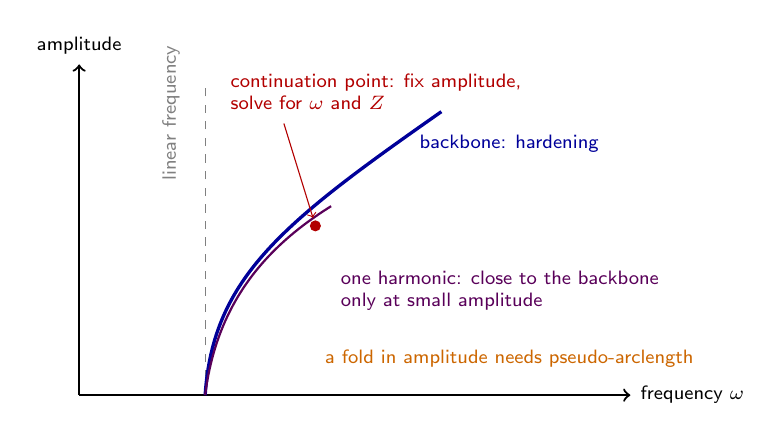
\begin{tikzpicture}[font=\sffamily\scriptsize]
\draw[->,thick] (0,0)--(7.0,0) node[right] {frequency $\omega$};
\draw[->,thick] (0,0)--(0,4.2) node[above] {amplitude};
\draw[dashed,gray] (1.6,0)--(1.6,4.0);
\node[gray,anchor=south west,rotate=90] at (1.4,2.6) {linear frequency};
\draw[blue!60!black,very thick] (1.6,0)..controls (1.7,1.5) and (2.6,2.2)..(4.6,3.6);
\node[blue!60!black,anchor=west] at (4.2,3.2) {backbone: hardening};
\draw[violet!70!black,thick] (1.6,0)..controls (1.75,1.2) and (2.4,1.9)..(3.2,2.4);
\node[violet!70!black,anchor=north west,align=left] at (3.2,1.7) {one harmonic: close to the backbone\\only at small amplitude};
\fill[red!70!black] (3.0,2.15) circle (2pt);
\draw[red!70!black,->] (2.6,3.45)--(2.97,2.25);
\node[red!70!black,anchor=south,align=center] at (4.2,3.9) {};
\node[red!70!black,anchor=south west,align=left] at (2.0,3.45) {};
\node[red!70!black,anchor=south west,align=left] at (1.8,3.5) {continuation point: fix amplitude,\\solve for $\omega$ and $\bm Z$};
\node[orange!80!black,anchor=north west,align=left] at (3.0,0.7) {a fold in amplitude needs pseudo-arclength};
\end{tikzpicture}
